\section{Análise Multivariada}

Eu fiz os dendogramas dos top 10, 20, 25, 50 e 100 municípios, tanto para o Wikiaves, quanto para o SpeciesLink. Acontece que, em certos momentos há empates: por exemplo, dois municípios em 100° possuem o mesmo número de espécies (no caso, por Jaccard ser uma distancia binária). Nesses casos, deixei com 102 municípios (há um empate de 4 municípios). Há algum \asp{critério de desempate}?

Essa tabela representa a correlação cofenética para cada um dos dendogramas, não está bem estabelecida como a tabela do artigo de Whisky que o senhor falou. É mais uma tabela de apoio para escolher um \asp{corte} entre a quantidade de municípios:

\begin{figure}[h!]
{\scriptsize Tabela 12. Correlação cofenética segundo o número de municípios. WAV = Wikiaves, SLI = SpeciesLink.}
\centering
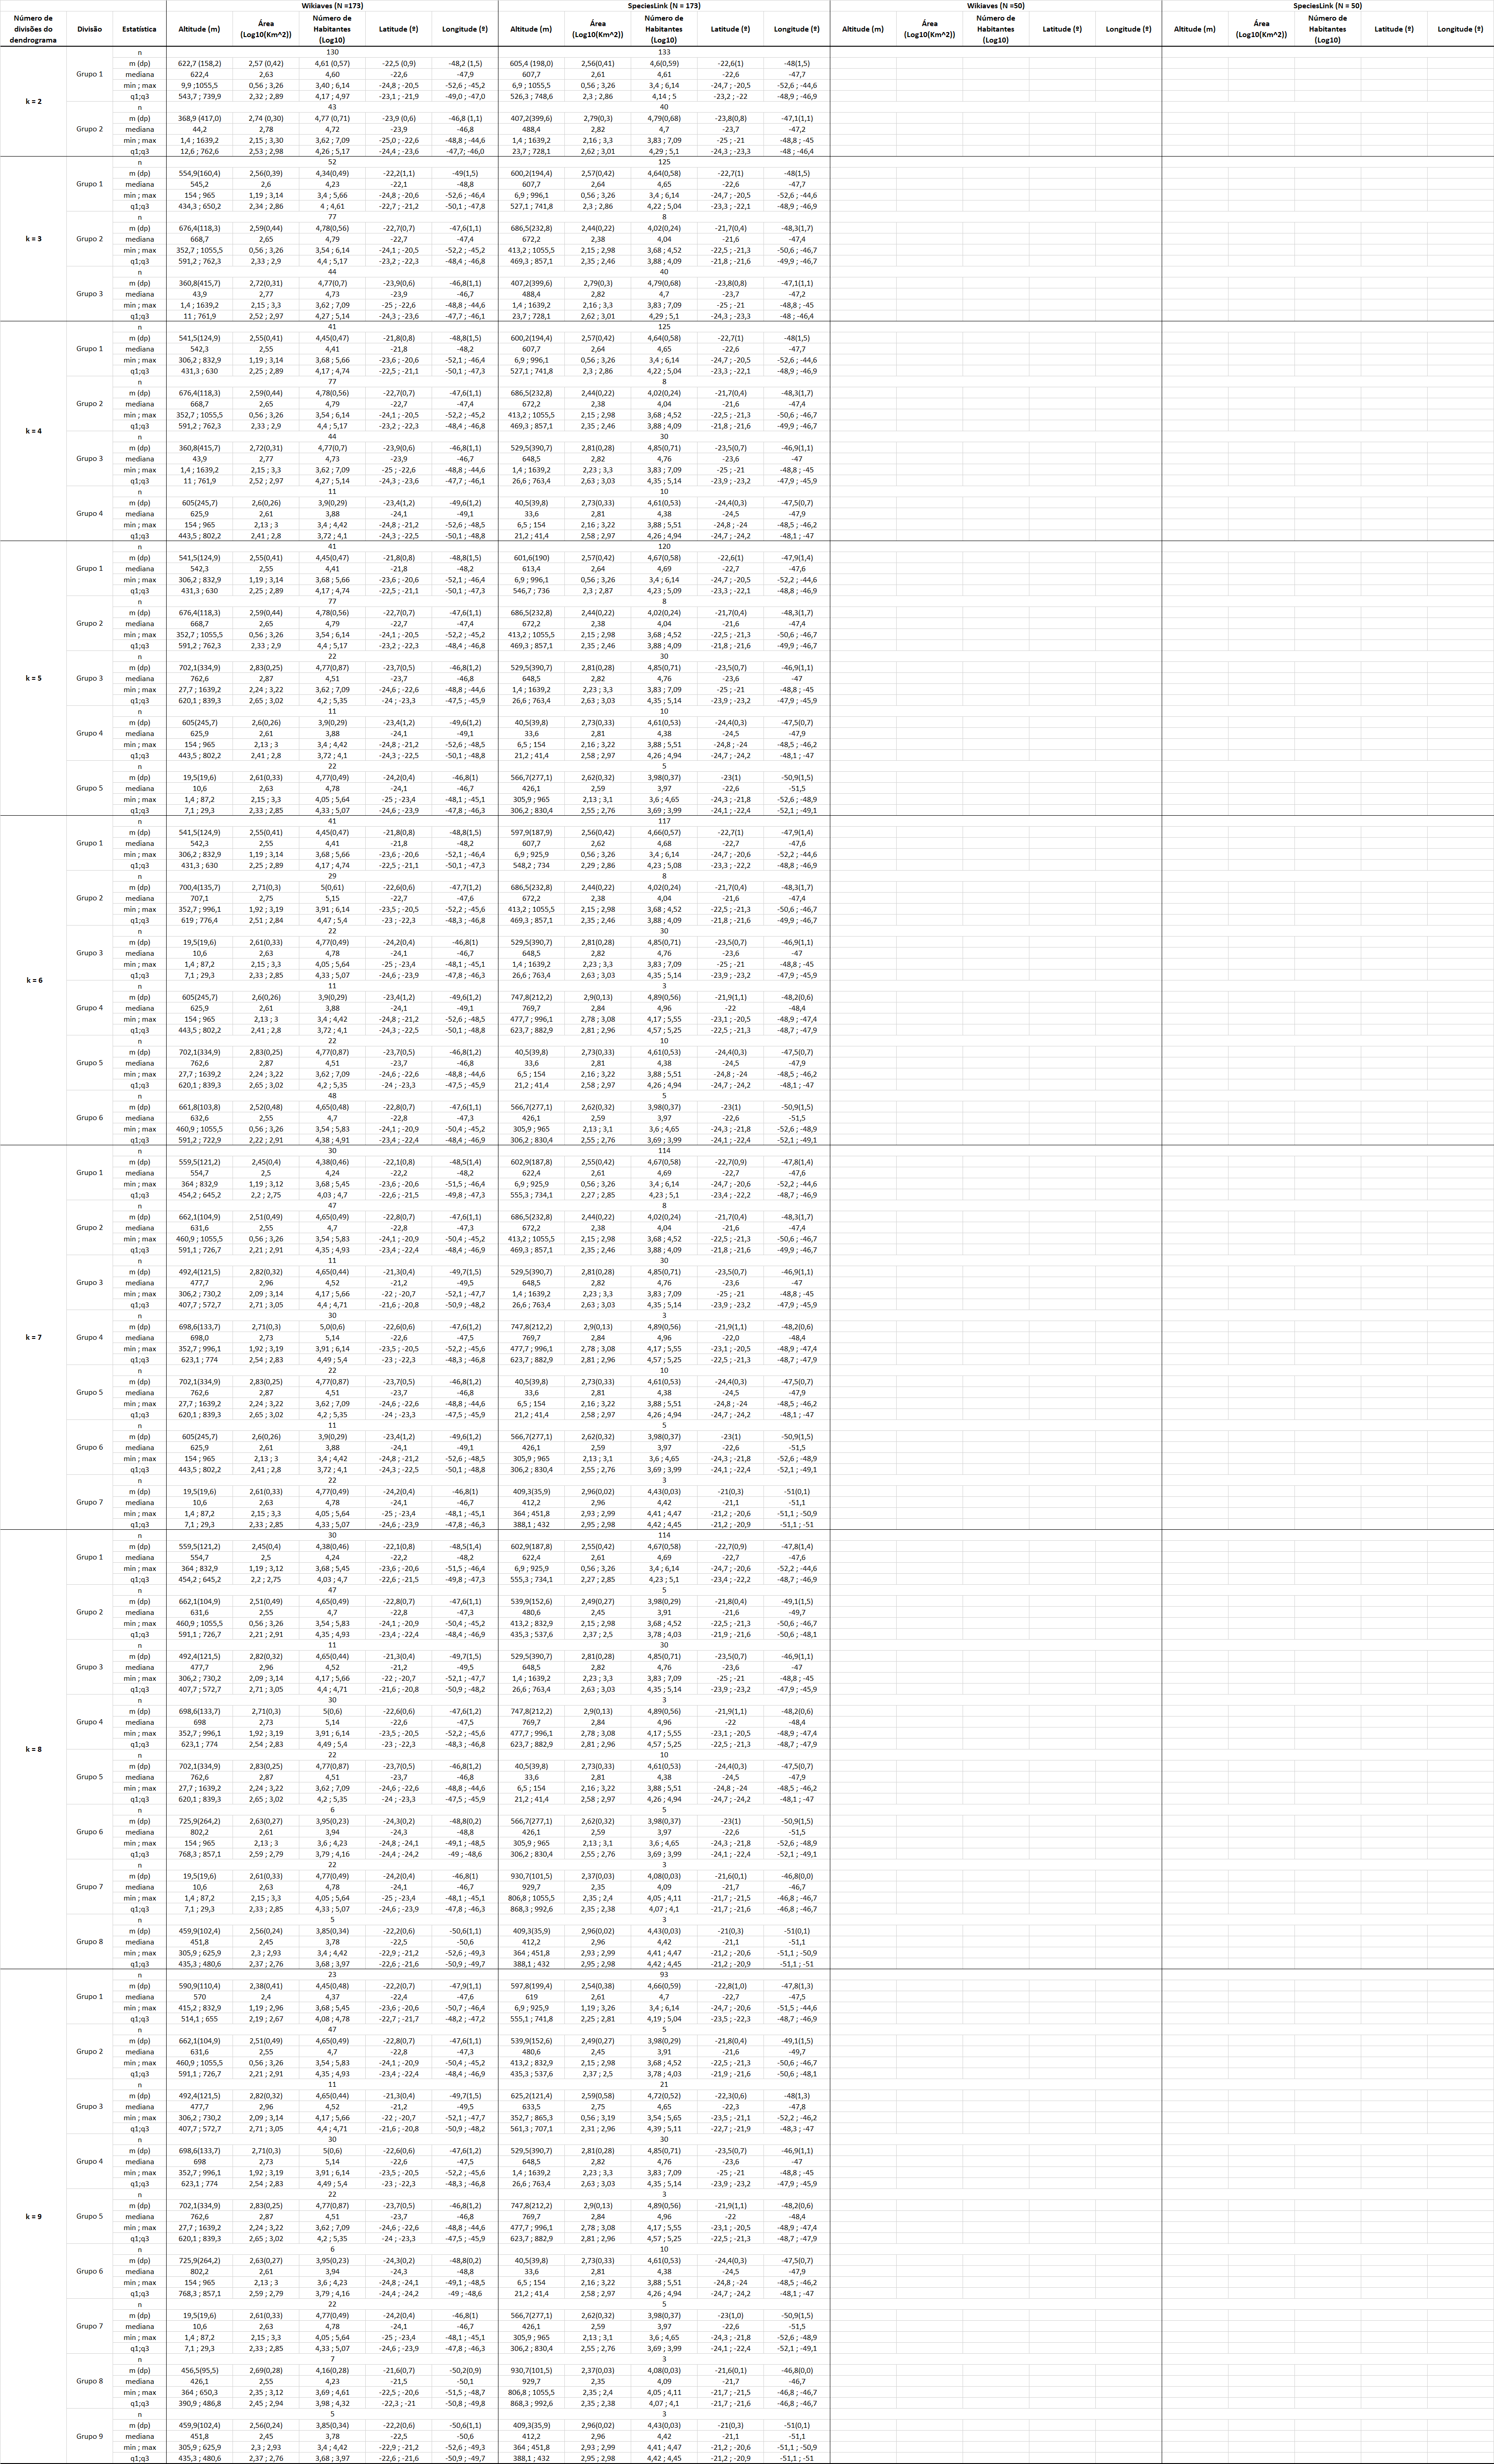
\includegraphics{Tabelas/12.png}
\end{figure}

Dendogramas: \href{https://github.com/bfaria1/ProjWAV/blob/master/Figuras.md}{https://github.com/bfaria1/ProjWAV/blob/master/Figuras.md}
